\documentclass[assignment02_Solutions]{subfiles}

\IfSubStr{\jobname}{\detokenize{Solutions}}{\toggletrue{solutions}}{\toggletrue{solutions}}

\fancypagestyle{firstpage}

{\rhead{Assignment 2 \linebreak \textit{Version: \today}}}

\title{Assignment 2: Probabilistic Graphical Models}
\author{Machine Learning}
\date{Fall 2019}

\begin{document}

\maketitle
\thispagestyle{firstpage}


\begin{learningobjectives}
\bi
\item TODO
\ei
\end{learningobjectives}

\section{Motivation and Context}
\bi
\item We’ve learned how probabilities can be used to describe uncertainty in the world
\item We’ve learned how Bayes' rule can be used to reason about hypotheses, models, or other things that cannot be directly observed.
\ei

\section{Product Rule and Marginalization for Random Variables}
\begin{recall}[Product Rule and Marginalization for Events]
Last assignment we learned about two very powerful techniques for computing the probability of events.
\bi
\item The first technique we learned was the product rule (or conjunction rule), which states that for any two events $\mathcal{A}$ and $\mathcal{B}$,
\begin{align}
p(\mathcal{A}, \mathcal{B}) &= p(\mathcal{A}) p(\mathcal{B}|\mathcal{A}) \label{eq:prodcutruleevents} \\
&= p(\mathcal{B}) p(\mathcal{A}|\mathcal{B}) \enspace  . \nonumber
\end{align}
\item The second technique we learned was marginalization.  This technique states that for any two events $\mathcal{A}$ and $\mathcal{B}$,
\begin{align}
p(\mathcal{A}) &= p(\mathcal{A}, \mathcal{B}) + p(\mathcal{A}, \neg \mathcal{B}) \label{eq:marginalizationevents}
\end{align}
\ei
\end{recall}

It turns out that these rules can modified slightly to apply to random variables as well (instead of just events).

\subsection{Product Rule for Random Variables}
Suppose we have two random variables $X$ and $Y$.  If we want to know the probability of random variable $X$ taking on value $x$ (it is common to use a lower case letter to refer to a particular value of a random variable) and random variable $Y$ simultaneously taking on value $y$ we can decompose it using the product rule in the following way.

\begin{align}
p(X = x, Y = y) &= p(X=x)p(Y=y | X=x) \\
&= p(Y=y)p(X=x|Y=y) \nonumber
\end{align}

Notice that this looks pretty much identical to Equation~\ref{eq:prodcutruleevents} with the exception that instead of referencing whether an event happens, we are now referencing a random variable taking on a particular value.

\begin{exercise}
Include some questions, perhaps on rolling dice or something of that nature.  Maybe something where things aren't conditionally independent could be cool to motivate the next section.
\end{exercise}

\subsection{Marginalization for Random Variables}
Again, suppose we have two random variables $X$ and $Y$.  We are interested in computing $p(X = x)$ through by marginalizing out the random variable $Y$.  For simplicity, let's assume that $Y$ can only take on integer values from 1 to $k$.  We can write marginal distribution $p(X=x)$ in the following way.

\begin{align}
p(X=x) &= \sum_{i=1}^k p(X=x, Y=i)\label{eq:rvmarginal}
\end{align}

You should notice that this equation is very similar to Equation~\ref{eq:marginalizationevents} except instead of summing over the probability for the two possible outcomes with respect to the event $\mathcal{B}$ (it could either happen or not), we are now summing over the $k$ possible values that $Y$ could take.  Of course random variables don't necessarily have to take on values from 1 to $k$.  In general if the random variable $Y$ can take on any value from some discrete set of values $\mathcal{Y}$ (we are using the calligraphic font because we are referring to a set), then the margin distribution of $X$ can be written as:
\begin{align}
p(X=x) &= \sum_{y \in \mathcal{Y}} p(X=x, Y=y) \enspace .
\end{align}
Notice that Equation~\ref{eq:rvmarginal} is a special case of the preceding equation where $\mathcal{Y} = \{1, 2, \ldots, k\}$.

\begin{exercise}
TODO
\end{exercise}

\section{Independence and Conditional Independence}

TODO Write intro explaining, in brief, what these two things are.

\subsection{Independence}
The product rule of probability can often be simplified when two events, $\mathcal{A}$ and $\mathcal{B}$ are independent.  As an example, suppose $\mathcal{A}$ represents the event that the first flip of a coin comes up heads and event $\mathcal{B}$ is the event that the second flip of the same coin comes up heads.  Since whether or not $\mathcal{A}$ occurs tells us nothing about whether $\mathcal{B}$ would occur, we say that $\mathcal{A}$ and $\mathcal{B}$ are independent events (we use the notation $\mathcal{A} \condindep \mathcal{B}$ to indicate that $\mathcal{A}$ is independent of $\mathcal{B}$).  An event $\mathcal{A}$ is independent of another event $\mathcal{B}$ if and only if the following condition holds.
\begin{align}
p(\mathcal{A}, \mathcal{B}) &= p(\mathcal{A}) p(\mathcal{B}) \label{eq:indepevents}
\end{align}

Another way to think about this is that if we hard started with the product rule $p(\mathcal{A}, \mathcal{B}) = p(\mathcal{A}) p(\mathcal{B} | \mathcal{A})$ we could have crossed out the conditioning on $\mathcal{A}$ from the second term since if two events are independent, knowing whether one happened doesn't change the probability of the other happening.

A very similar equation to Equation~\ref{eq:indepevents} can be defined for random variables.  Two random variables $X$ and $Y$ are independent if and only if the following condition holds for any values $x$ and $y$.

\begin{align}
p(X=x, Y=y) &= P(X=x) p(Y=y | X=x)
\end{align}

\begin{exercise}
Give examples of events that are or are not independent.

Give examples of random variables that are or are not independent.
\end{exercise}

\subsection{Conditional Independence}
Sometimes two events (or two random variables) that are not independent might become independent when conditioned on another event.  As a motivating example, consider a variant of the coin problem we saw last assignment.  A bag contains two coins ($\mathcal{C}_1$ and $\mathcal{C}_2$).  Coin 1 is fair $p(\mathcal{H} | \mathcal{C}_1) = \frac{1}{2}$.  Coin 2 is not fair ($p(\mathcal{H} | \mathcal{C}_2) = \frac{4}{5}$).  Suppose we choose one of the two coins with equal probability.  Let $\mathcal{C}_1$ represents the event that we choose coin 1 and $\mathcal{C}_2$ represent the event that we choose coin 2.  We then flip the coin twice.  Let $\mathcal{H}_1$ represent the event that the first flip comes up heads and $\mathcal{H}_2$ represent the event that the second flip comes up heads.  The question is are $\mathcal{H}_1$ and $\mathcal{H}_2$ independent (i.e., is $\mathcal{H}_1 \condindep \mathcal{H}_2$)?

\begin{exercise}
In order to determine whether $\mathcal{H}_1 \condindep \mathcal{H}_2$, let's make a tree diagram of the situation.
\begin{center}
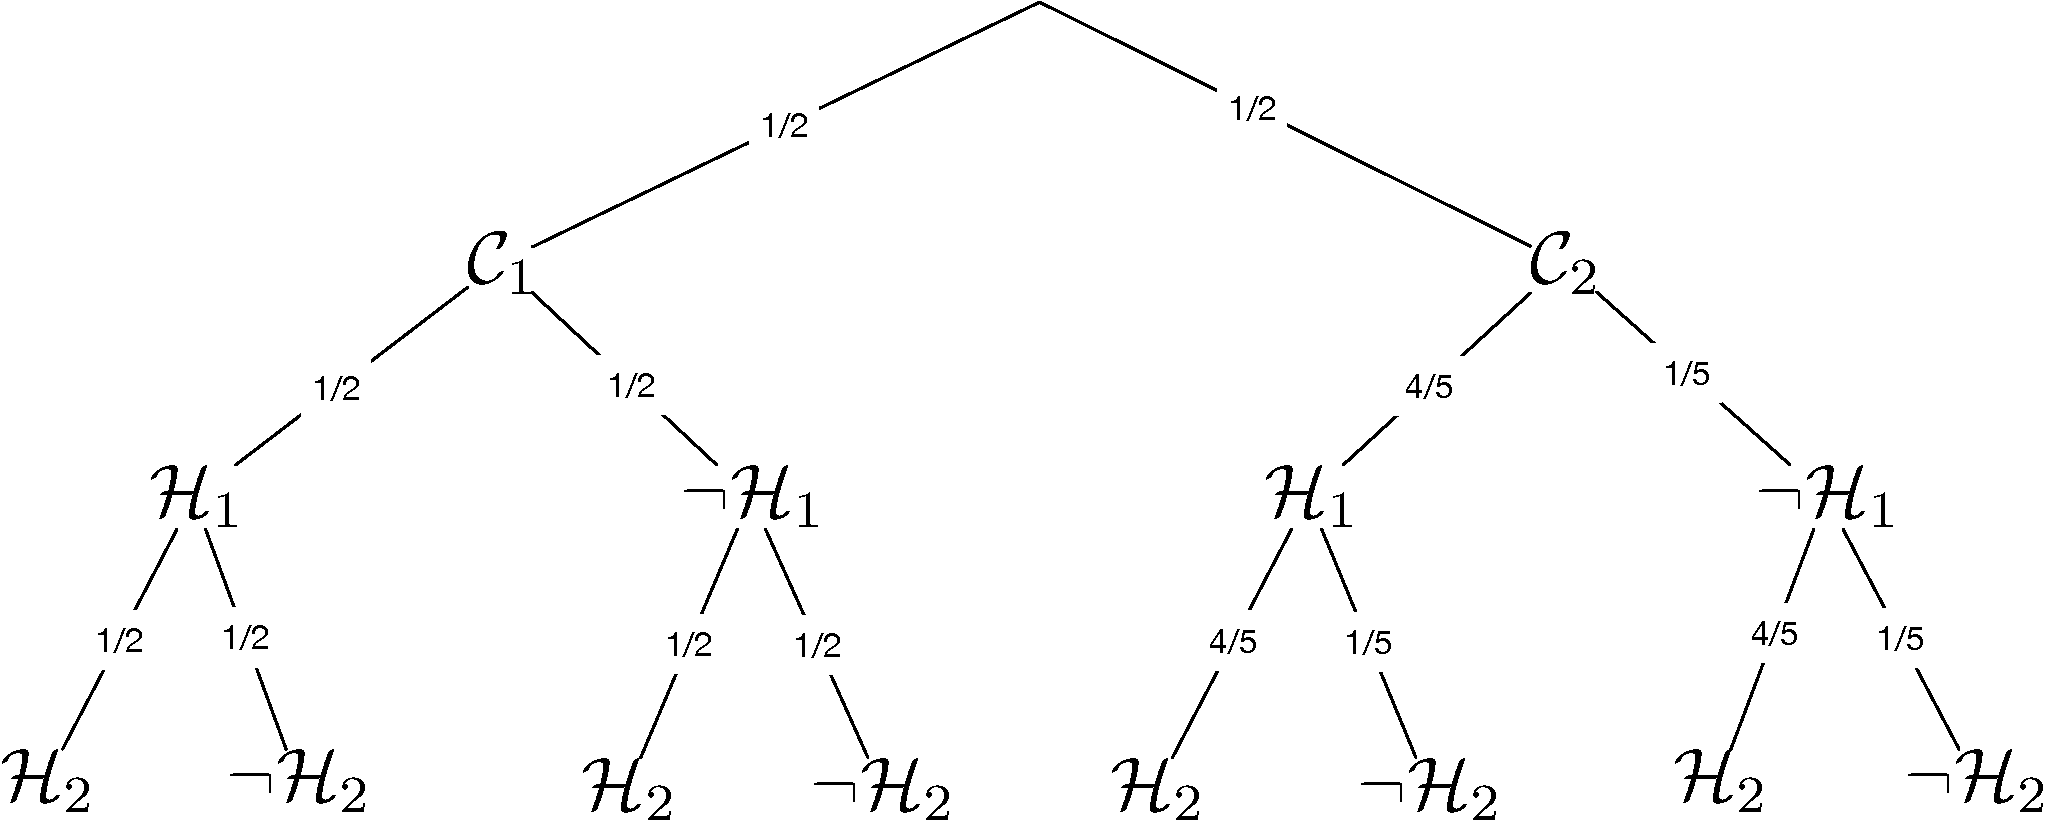
\includegraphics[width=\linewidth]{figures/twocoins}
\end{center}
Given the tree diagram above, is $\mathcal{H}_1 \condindep \mathcal{H}_2$?

\begin{boxedsolution}
In order to test $\mathcal{H}_1 \condindep \mathcal{H}_2$ we need to check the following condition:
\begin{align}
p(\mathcal{H}_1, \mathcal{H}_2) \stackrel{?}{=} p(\mathcal{H}_1) p(\mathcal{H}_2)
\end{align}

We can compute each of the terms in the preceding equation using the tree diagram.  In total there are 8 possible paths through the tree.  Recall that we can find the probability of a path by multiplying the numbers on the arrows.  To find the probability of a particular event, say $p(\mathcal{H}_1)$ we just add up the probability of all of the paths that include $\mathcal{H}_1$.  We can apply this technique to each of the events we care about.
\begin{align}
p(\mathcal{H}_1) &= p(\mathcal{C}_1, \mathcal{H}_1, \mathcal{H}_2) +  p(\mathcal{C}_1, \mathcal{H}_1, \neg \mathcal{H}_2)+  p(\mathcal{C}_2, \mathcal{H}_1, \mathcal{H}_2) +  p(\mathcal{C}_2, \mathcal{H}_1, \neg \mathcal{H}_2) \nonumber \\
&= \left ( \frac{1}{2} \times \frac{1}{2} \times \frac{1}{2}  \right) + \left ( \frac{1}{2} \times \frac{1}{2} \times \frac{1}{2} \right ) + \left ( \frac{1}{2} \times \frac{4}{5} \times \frac{4}{5}  \right) + \left ( \frac{1}{2} \times \frac{4}{5} \times \frac{1}{5} \right )\nonumber \\
&= \frac{13}{20} \nonumber \\
p(\mathcal{H}_2) &= p(\mathcal{C}_1, \mathcal{H}_1, \mathcal{H}_2) +  p(\mathcal{C}_1, \neg \mathcal{H}_1, \mathcal{H}_2)+  p(\mathcal{C}_2, \mathcal{H}_1, \mathcal{H}_2) +  p(\mathcal{C}_2, \neg \mathcal{H}_1, \mathcal{H}_2) \nonumber \\
&= \left ( \frac{1}{2} \times \frac{1}{2} \times \frac{1}{2}  \right) + \left ( \frac{1}{2} \times \frac{1}{2} \times \frac{1}{2} \right ) + \left ( \frac{1}{2} \times \frac{4}{5} \times \frac{4}{5}  \right) + \left ( \frac{1}{2} \times \frac{1}{5} \times \frac{4}{5} \right )\nonumber \\
&= \frac{13}{20} \nonumber \\
p(\mathcal{H}_1, \mathcal{H}_2) &=  p(\mathcal{C}_1, \mathcal{H}_1, \mathcal{H}_2) + p(\mathcal{C}_2, \mathcal{H}_1, \mathcal{H}_2) \nonumber \\
&= \left ( \frac{1}{2} \times \frac{1}{2} \times \frac{1}{2} \right ) + \left ( \frac{1}{2} \times \frac{4}{5} \times \frac{4}{5} \right ) \nonumber \\
&= \frac{89}{200} \nonumber \\
p(\mathcal{H}_1) p(\mathcal{H}_2) &= \frac{13}{20} \times \frac{13}{20} = \frac{169}{400} \neq \frac{89}{200} = p(\mathcal{H}_1, \mathcal{H}_2) \nonumber
\end{align}
Since $p(\mathcal{H}_1, \mathcal{H}_2) \neq p(\mathcal{H}_1) p(\mathcal{H}_2)$, $\mathcal{H}_1$ is not independent of $\mathcal{H}_2$.
\end{boxedsolution}
\end{exercise}

It turns out that even though $\mathcal{H}_1$ and $\mathcal{H}_2$ are not independent, we can state that they are what's called \emph{conditionally independent} given $\mathcal{C}_1$ (or $\mathcal{C}_2$).  More formally, events $\mathcal{A}$ and $\mathcal{B}$ are considered conditionally independent given $\mathcal{C}$ (written as $\mathcal{A} \condindep \mathcal{B}~|~\mathcal{C}$) if and only if

\begin{align}
p(\mathcal{A}, \mathcal{B} | \mathcal{C}) &= p(\mathcal{A} | \mathcal{C}) p(\mathcal{B} | \mathcal{C}) \nonumber
\end{align}

\begin{exercise}
\bes
\item Show that $\mathcal{H}_1 \condindep \mathcal{H}_2~|~\mathcal{C}_1$
\begin{boxedsolution}
We need to show that $p(\mathcal{H}_1 , \mathcal{H}_2 | \mathcal{C}_1) = p(\mathcal{H}_1 | \mathcal{C}_1) p(\mathcal{H}_2 | \mathcal{C}_1)$.  We can use the tree diagram to compute these conditional probabilities by starting our multiplication after the branch that we are conditioning on.
\begin{align}
p(\mathcal{H}_1 , \mathcal{H}_2 | \mathcal{C}_1)  &= \frac{1}{2} \times \frac{1}{2} = \frac{1}{4} \nonumber \\
p(\mathcal{H}_1 | \mathcal{C}_1) &= p(\mathcal{H}_1, \mathcal{H}_2 | \mathcal{C}_1) + p(\mathcal{H}_1, \neg \mathcal{H}_2 | \mathcal{C}_1) \nonumber \\
&= \left ( \frac{1}{2} \times \frac{1}{2} \right) + \left ( \frac{1}{2} \times \frac{1}{2} \right) = \frac{1}{2} \nonumber \\
p(\mathcal{H}_2 | \mathcal{C}_1) &= p(\mathcal{H}_1, \mathcal{H}_2 | \mathcal{C}_1) + p(\neg \mathcal{H}_1,  \mathcal{H}_2 | \mathcal{C}_1) \nonumber \\
&= \left ( \frac{1}{2} \times \frac{1}{2} \right) + \left ( \frac{1}{2} \times \frac{1}{2} \right) = \frac{1}{2} \nonumber \\
p(\mathcal{H}_1 , \mathcal{H}_2 | \mathcal{C}_1) &=  \frac{1}{2} \times \frac{1}{2} \nonumber \\
&= p(\mathcal{H}_1 | \mathcal{C}_1) p(\mathcal{H}_2 | \mathcal{C}_1) \nonumber
\end{align}
\end{boxedsolution}
\item Show that $\mathcal{H}_1 \condindep \mathcal{H}_2~|~\mathcal{C}_2$

\begin{boxedsolution}
We need to show that $p(\mathcal{H}_1 , \mathcal{H}_2 | \mathcal{C}_2) = p(\mathcal{H}_1 | \mathcal{C}_2) p(\mathcal{H}_2 | \mathcal{C}_2)$.  We can use the tree diagram to compute these conditional probabilities by starting our multiplication after the branch that we are conditioning on.
\begin{align}
p(\mathcal{H}_1 , \mathcal{H}_2 | \mathcal{C}_2)  &= \frac{4}{5} \times \frac{4}{5} = \frac{16}{25} \nonumber \\
p(\mathcal{H}_1 | \mathcal{C}_2) &= p(\mathcal{H}_1, \mathcal{H}_2 | \mathcal{C}_2) + p(\mathcal{H}_1, \neg \mathcal{H}_2 | \mathcal{C}_2) \nonumber \\
&= \left ( \frac{4}{5} \times \frac{4}{5} \right) + \left ( \frac{4}{5} \times \frac{1}{2} \right) = \frac{4}{5} \nonumber \\
p(\mathcal{H}_2 | \mathcal{C}_2) &= p(\mathcal{H}_1, \mathcal{H}_2 | \mathcal{C}_2) + p(\neg \mathcal{H}_1,  \mathcal{H}_2 | \mathcal{C}_2) \nonumber \\
&= \left ( \frac{4}{5} \times \frac{4}{5} \right) + \left ( \frac{1}{5} \times \frac{4}{5} \right) = \frac{4}{5} \nonumber \\
p(\mathcal{H}_1 , \mathcal{H}_2 | \mathcal{C}_1) &=  \frac{4}{5} \times \frac{4}{5} \nonumber \\
&= p(\mathcal{H}_1 | \mathcal{C}_2) p(\mathcal{H}_2 | \mathcal{C}_2) \nonumber
\end{align}
\end{boxedsolution}
\ees
\end{exercise}

The definition of the conditional independence of events can be easily extended to random variables.  We say that random variables $X$ and $Y$ are conditionally independent given random variable $Z$ (i.e., $X \condindep Y ~|~ Z$) if and only if the following equation holds for all $x, y, z$.

\begin{align}
p(X=x,Y=y | Z=z) &= p(X=x|Z=z) p(Y=y|Z=z)
\end{align}

\section{Bayesian Networks}

The calculations in the previous section were a bit tedious.  It would be great if there was some way to reason about the conditional independence properties of two random variables conditioned on some other random variable.  Luckily... drum roll... there is!  A Bayesian network (sometimes called a Bayesian belief network or a probabilistic directed acyclic graphical model) represents the conditional independence relationships between random variables through a graphical, causal structure.  We'll use BN as shorthand for ``Bayesian network.''  Take for instance, the BN that represents the coin problem that we did in the last section. (TODO: maybe redo this notation to remove the T's and F's).

\begin{center}
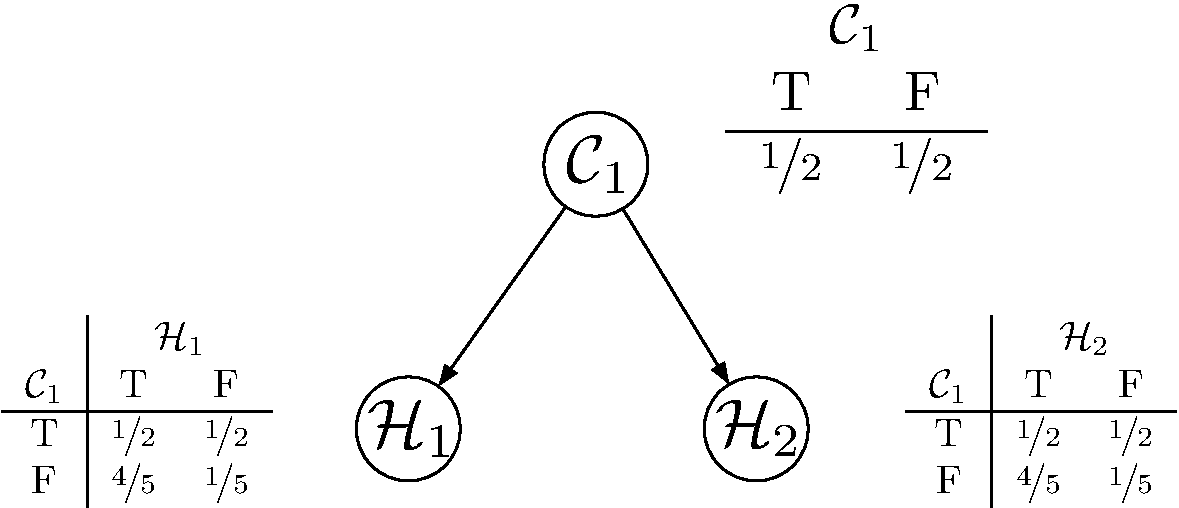
\includegraphics[width=0.6\linewidth]{figures/coinbn}
\end{center}

The graphical structure (edges and nodes in the graph) tell us everything we need to infer the conditional independence properties in the graph (Note that we haven't told you how you can extract this information from the graph.  That's coming later in the assignment).  The tables that are listed by each node tell us the probability of the event happening versus not happening conditioned on whether or not the events listed on the nodes parents\sidenote{You may not be familiar with the idea of the ``parents'' of a node in a graph.  A node $A$ is the parent of a node $B$ if there is an edge directly connecting them that points from $A$ to $B$} happened (happening \emph{T} stands for \emph{True} or that the event does happen and \emph{F} stands for \emph{False} or that the event does not happen).

The BN provides us with a way of computing any relevant probability (e.g., marginal, conditional, joint) for the nodes in the network.  The condition that must hold for any BN is that if we want to write the joint distribution of all of the events or random variables (the relationship is the same for either) in the network, it must factorize in the following way.  We'll use $X_1, X_2, \ldots X_n$ to represent random variables in the network and we'll define the function $Pa(X_i)$ to return all of the random variables that are parents of $X_i$.

\begin{align}
p(X_1, X_2, \ldots, X_n) &= p(X_1 | Pa(X_1)) \times p(X_2 | PaX_2)) \times \ldots p(X_n | Pa(X_n)) 
\end{align}

Back to our coin BN, this means that we can write the joint distribution like so.

\begin{align}
p(\mathcal{C}_1, \mathcal{H}_1, \mathcal{H}_2) = p(\mathcal{C}_1) p(\mathcal{H}_1 | \mathcal{C}_1) p(\mathcal{H}_2 | \mathcal{C}_1) \nonumber
\end{align}

\begin{exercise}
Consider the belief network below (source: \url{https://en.wikipedia.org/wiki/Bayesian_network\#Example}). (TODO: not crazy about this notation)
\begin{center}
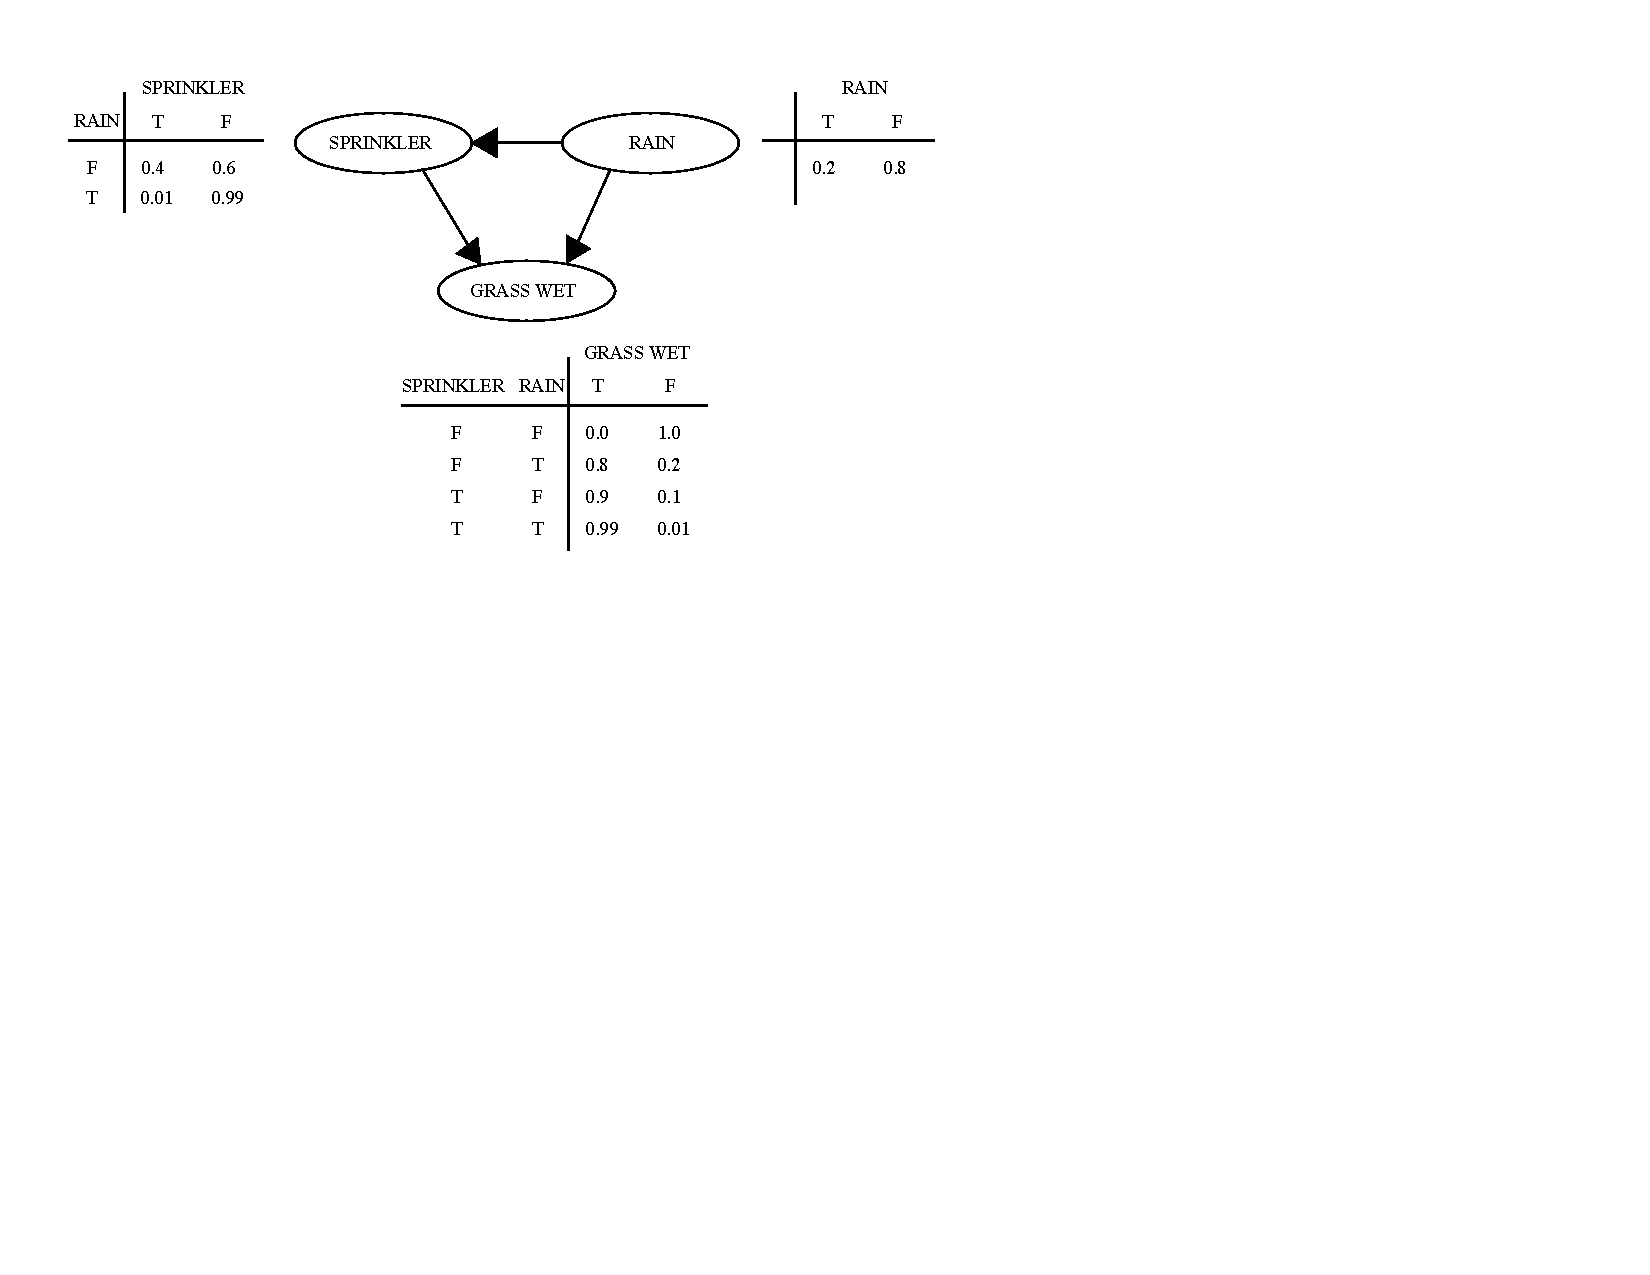
\includegraphics[width=0.7\linewidth]{figures/SimpleBayesNet}
\end{center}

Compute the following probabilities (for brevity we'll use the first letter of each node to indicate that the corresponding event happens (i.e., is true)).
\bes
\item $p(\mathcal{R}, \mathcal{G}, \neg \mathcal{S})$
\begin{boxedsolution}
\begin{align}
p(\mathcal{R}, \mathcal{G}, \neg \mathcal{S}) &= p(\mathcal{R}) p(\neg \mathcal{S} | \mathcal{R}) p(\mathcal{G} | \mathcal{R}, \neg \mathcal{S}) \nonumber \\
&= 0.2 \times 0.99 \times 0.8 \nonumber \\
&= 0.1584 \nonumber
\end{align}
\end{boxedsolution}
\item $p(\mathcal{R})$
\begin{boxedsolution}
This one is kind of a trick question.  Since $\mathcal{R}$ has no parents, we can just read the probability right off the probability table for the $\mathcal{R}$ node.  The answer is $0.2$.
\end{boxedsolution}
\item $p(\neg \mathcal{G}, \neg \mathcal{S})$ (hint: marginalize over $\mathcal{R}$)

\begin{boxedsolution}
\begin{align}
p(\neg \mathcal{G}, \neg \mathcal{S}) &= p(\neg \mathcal{G}, \neg \mathcal{S}, \mathcal{R}) + p(\neg \mathcal{G}, \neg \mathcal{S}, \neg \mathcal{R}) \nonumber \\
&= p(\mathcal{R}) p(\neg \mathcal{S} | \mathcal{R}) p (\neg \mathcal{G} | \mathcal{R}, \neg \mathcal{S} ) + p(\neg \mathcal{R}) p(\neg \mathcal{S} | \neg \mathcal{R}) p (\neg \mathcal{G} | \neg \mathcal{R}, \neg \mathcal{S} ) \nonumber \\
&= \left ( 0.2 \times 0.99 \times 0.2 \right ) + \left ( 0.8 \times 0.6 \times 1.0 \right ) \nonumber \\
&= 0.5196 \nonumber
\end{align}
\end{boxedsolution}

\ees

\end{exercise}

\subsection{D-separation}
While the graphical structure of the BN is useful for decomposing the joint distribution of the random variables in the graph, it can also be used to reason about the conditional independence relationships in the graph.  For instance, it's possible that given the BN for the coin problem that we can determine that $\mathcal{H}_1 \condindep \mathcal{H}_2~|~\mathcal{C}_1$ simply by looking at the graph.  In order to figure out these sorts of conditional independence relationships, we need to learn about the concept of d-separation.

\begin{externalresources}
\bi
\item Read \href{http://bayes.cs.ucla.edu/BOOK-09/ch11-1-2-final.pdf}{d-Separation without Tears}.
\item \href{https://www.youtube.com/watch?v=IjoWqnH6HmU}{This one seems pretty good}
\item \href{https://www.youtube.com/watch?v=yDs_q6jKHb0}{Pieter Abbeel Lecture} (not sure how clear this is)
\ei
\end{externalresources}

\begin{exercise}
Consider the following BN that describes how two people John and Mary respond to an alarm going off in their apartment building.  In this case the alarm is triggered either by an earthquake, a burglary, or might go off on accident.
\vspace{1em}
\begin{center}
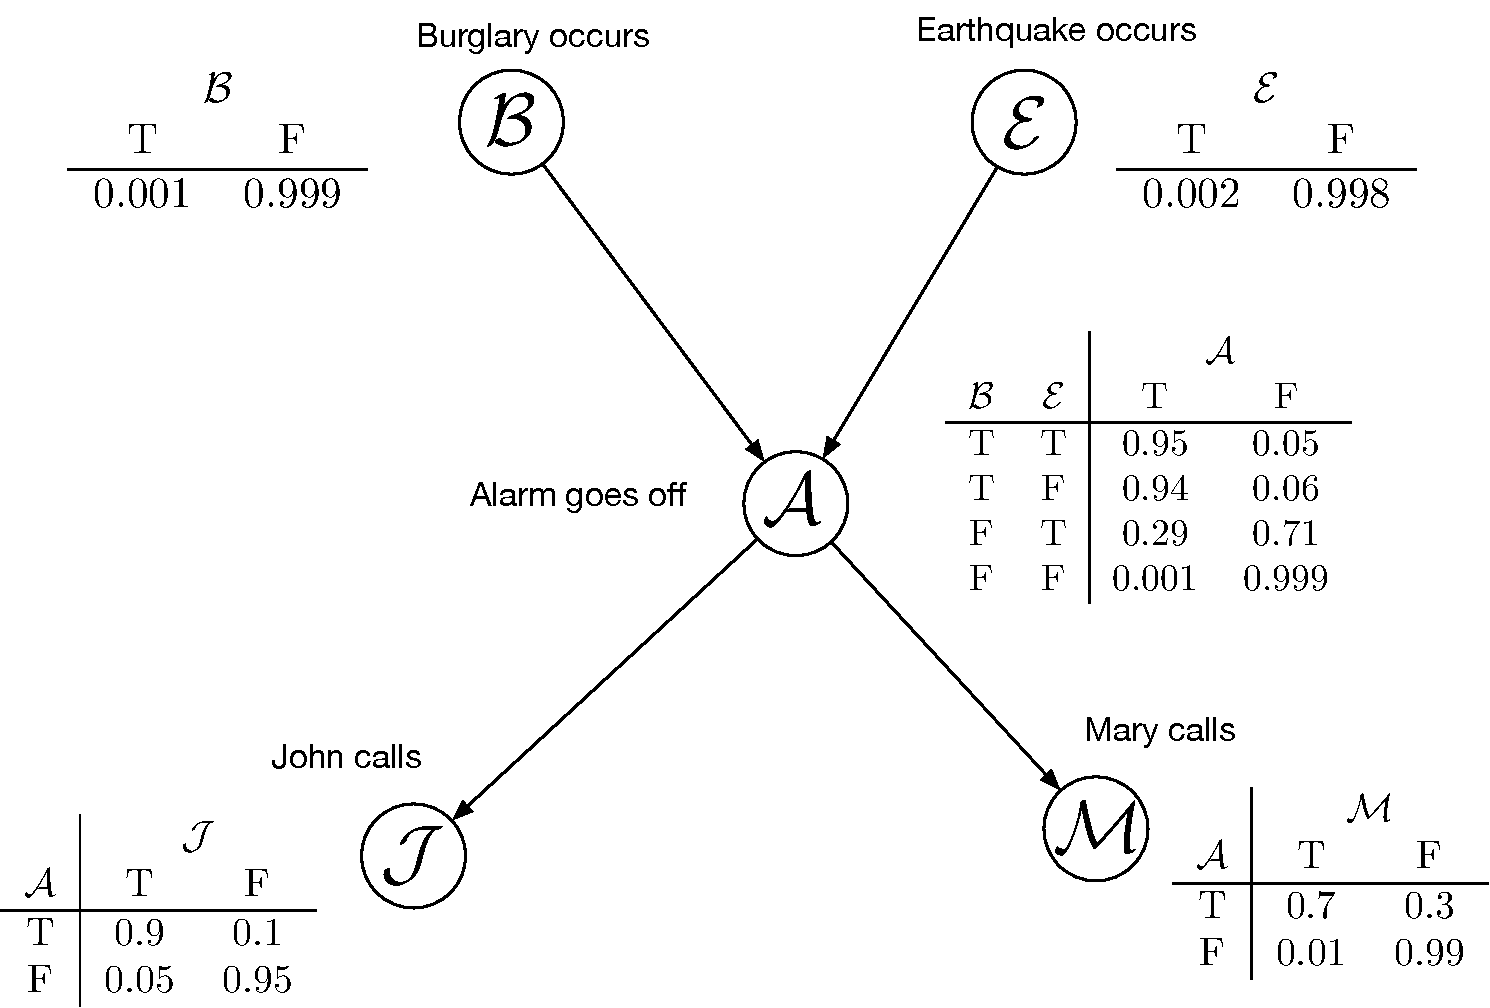
\includegraphics[width=0.8\linewidth]{figures/maryjohn}
\end{center}

Compute the following probabilities (for some problems you will be able to simplify your calculations by testing for the independence (or conditional independence) using d-separation.

\bes
\item $p(\mathcal{B}, \mathcal{E})$

\begin{boxedsolution}
$\mathcal{B}$ and $\mathcal{E}$ are d-separated by $\mathcal{A}$.  Therefore, $\mathcal{B} \condindep \mathcal{E}$.
\begin{align}
p(\mathcal{B}, \mathcal{E}) &= p(\mathcal{B}) p(\mathcal{A}) \nonumber \\
&= 0.001 \times 0.002 \nonumber \\
&= 0.000002 \nonumber
\end{align}
\end{boxedsolution}

\item $p(\mathcal{J}, \mathcal{M} | \mathcal{A})$

\begin{boxedsolution}
$\mathcal{J}$ and $\mathcal{M}$ are d-separated when conditioning on $\mathcal{A}$ (since it breaks path connecting them).  Therefore $\mathcal{J} \condindep \mathcal{M}~|~\mathcal{A}$.

\begin{align}
p(\mathcal{J}, \mathcal{M} | \mathcal{A}) &= p(\mathcal{J} | \mathcal{A}) p(\mathcal{M} | \mathcal{A}) \nonumber \\
&= 0.9 \times 0.7 \nonumber \\
&= 0.63 \nonumber
\end{align}
\end{boxedsolution}

\item $p(\mathcal{B} | \mathcal{A})$ (hint: don't forget about Bayes' rule) (hint 2: don't forget about marginalization)

\begin{boxedsolution}
If we marginalize our $\mathcal{E}$ we are left with the following.

\begin{align}
p(\mathcal{B} | \mathcal{A}) &= \frac{p(\mathcal{A} | \mathcal{B}) p(\mathcal{B})}{p(\mathcal{A})} \nonumber \\
p(\mathcal{A} | \mathcal{B}) &= p(\mathcal{A}, \mathcal{E} | \mathcal{B}) + p(\mathcal{A}, \neg \mathcal{E} | \mathcal{B}) \nonumber \\
&= p(\mathcal{E} | \mathcal{B}) p(\mathcal{A} | \mathcal{E}, \mathcal{B}) + p(\neg \mathcal{E} | \mathcal{B}) p(\mathcal{A} | \neg \mathcal{E}, \mathcal{B}) \nonumber \\
&=  p(\mathcal{E}) p(\mathcal{A} | \mathcal{E}, \mathcal{B}) + p(\neg \mathcal{E}) p(\mathcal{A} | \neg \mathcal{E}, \mathcal{B}) \nonumber \\
&= 0.002 \times 0.95 + 0.998 \times 0.94 \nonumber \\
&= 0.94002 \nonumber \\
p(\mathcal{A}) &= p(\mathcal{B}, \mathcal{E}, \mathcal{A}) +  p(\mathcal{B}, \neg \mathcal{E}, \mathcal{A}) + p(\neg \mathcal{B}, \mathcal{E}, \mathcal{A}) + p(\neg \mathcal{B}, \neg \mathcal{E}, \mathcal{A}) \nonumber \\
&= p(\mathcal{B}) p(\mathcal{E} | \mathcal{B}) p(\mathcal{A} | \mathcal{B}, \mathcal{E}) +   p(\mathcal{B}) p(\neg \mathcal{E} | \mathcal{B}) p(\mathcal{A} | \mathcal{B}, \neg \mathcal{E}) \nonumber \\
 &\hspace{0.5in} + p(\neg \mathcal{B}) p(\mathcal{E} | \neg \mathcal{B}) p(\mathcal{A} | \neg \mathcal{B}, \mathcal{E}) +  p(\neg \mathcal{B}) p(\neg \mathcal{E} | \neg \mathcal{B}) p(\mathcal{A} | \neg \mathcal{B}, \neg \mathcal{E}) \nonumber \\
 &= p(\mathcal{B}) p(\mathcal{E}) p(\mathcal{A} | \mathcal{B}, \mathcal{E}) +   p(\mathcal{B}) p(\neg \mathcal{E}) p(\mathcal{A} | \mathcal{B}, \neg \mathcal{E}) \nonumber \\
 &\hspace{0.5in} + p(\neg \mathcal{B}) p(\mathcal{E}) p(\mathcal{A} | \neg \mathcal{B}, \mathcal{E}) +  p(\neg \mathcal{B}) p(\neg \mathcal{E}) p(\mathcal{A} | \neg \mathcal{B}, \neg \mathcal{E}) \nonumber
\end{align}
\end{boxedsolution}

\item $p(\mathcal{B} | \mathcal{A}, \mathcal{E})$ (this is known as the phenomenon of \emph{explaining away})

\begin{boxedsolution}
\end{boxedsolution}

\ees
\end{exercise}

\section{Generative versus Discriminative Models}
TODO: write some intro here

\subsection{Discriminative Models: a Look Back at Logistic Regression}

Let's take a minute and think back to the logistic regression model for binary classification that we learned about in module 1.  Given an input point $\mathbf{x_i}$, the logistic regression utilized a weight vector $\mathbf{w}$ to compute the probability that the corresponding output $y_i$ was 1 using the $\sigma(\mathbf{w}^\top \mathbf{x_i}) = \frac{1}{1+e^{-\mathbf{w}^\top \mathbf{x_i}}}$ (recall that $\sigma$ is known as the sigmoid function and serves to squash its input into a number between 0 and 1, which can serve as a valid probability).  While we didn't quite have the vocabulary for it then, what we really doing at the time was computing a conditional probability.  We can think of $Y_i$ as a random variable that represents the output that corresponds to the the input point $\mathbf{x_i}$ ($Y_i$ is either 0 or 1 since we are dealing with binary classification).  We can also think of the input as a random variable $\mathbf{X_i}$ (thinking of the input in this way will be helpful later in this section).  In this way, we can think of what the logistic regression algorithm is doing as computing the following conditional probability:
\begin{align}
p(Y_i = 1 | X_i = \mathbf{x_i}) &= \sigma(\mathbf{w}^\top \mathbf{x_i}) \enspace .
\end{align}

We then defined a loss function that would let us find the best weights, $\mathbf{w}$, given a training set of corresponding input output pairs $(\mathbf{x_1}, y_1), (\mathbf{x_2}, y_2), \ldots, (\mathbf{x_n}, y_n)$.  The details of how we did this are not important to the point we are trying to make now, so it'll suffice to say that learning in a logistic regression model meant tuning the conditional distribution of the outputs (the $Y_i$'s) given the inputs ($\mathbf{x_i}$'s) to fit the training data the best.  This type of model is what is known as a \emph{discriminative model} (the \href{https://en.wikipedia.org/wiki/Discriminative_model}{Wikipedia article on discriminative models} has more details if you are interested).

\vspace{1em}

\begin{understandingcheck}
TODO
\end{understandingcheck}

\subsection{Generative Models}
While the approach outlined above is totally logical, it is not the only way to approach supervised machine learning.  Using a simple application of Bayes' rule, we can derive a whole new approach to the problem!  Since we are interested in predicting $Y_i$ given some inputs $\mathbf{x_i}$ it of course makes sense, for example for a binary classification problem, to want to determine $p(Y_i = 1 | \mathbf{x_i})$.  Instead of modeling that distribution directly, we can instead use Bayes' rule to transform this probability distribution.

TODO: not sure if we should introduce a convention along the lines of $p(\mathbf{x_i}) = p(X_i = \mathbf{x_i})$.

\begin{align}
p(Y_i  = 1 | X_i = \mathbf{x_i}) &= \frac{p(X_i = \mathbf{x_i} | Y_i = 1) p(Y_i = 1)}{p(X_i = \mathbf{x_i})} \label{eq:pgm} \\
&= \frac{p(X_i = \mathbf{x_i} | Y_i = 1) p(Y_i = 1)}{p(X_i =  \mathbf{x_i} | Y_i = 1) p(Y_i = 1) + p(X_i = \mathbf{x_i} | Y_i = 0) p(Y_i = 0)} \nonumber
\end{align}

\begin{marginfigure}
\begin{center}
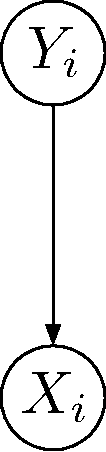
\includegraphics[width=0.2\linewidth]{figures/pgm}
\end{center}
\caption{The graphical model corresponding to a probabilistic generative model in which the latent variable $Y_i$ is thought of as a causally generating $X_i$.\label{fig:pgm}}
\end{marginfigure}

What these equations are telling us is that if we have a model of the probability of the output being 1 \emph{a priori} ($p(Y_i = 1)$) along with a model of the inputs $\mathbf{x_i}$ given the output $Y_i$ ($p(Y_i | \mathbf{x_i})$), then we have all the information we need to compute $p(Y_i = 1 | \mathbf{x}_i)$.  In a way this amounts to adopting the perspective that the hidden output $Y_i$ causes the input $X_i$ (see Figure~\ref{fig:pgm}).  We call this sort of model a \href{https://en.wikipedia.org/wiki/Generative_model}{probabilistic generative model}.

The natural question you might ask yourself is \emph{why?} Here are some potential advantages of using probabilistic generative models.
\bi
\item Suppose you found out that $p(Y_i)$ changed for some reason (any thoughts on when this might happen?  Post here on NB).  Incorporating this change into a probabilistic graphical model would be very straight forward (just modify $p(Y_i =1)$ in Equation~\ref{eq:pgm}).
\item Suppose you found out that $p(X_i | Y_i)$ changed for some reason.  For example, if one of the elements of $X_i$ represents a result obtained by running some sort of medical test, the sensitivity of that medical test might change (any other examples on when this might happen? Post here on NB.).
\item Suppose that instead of classifying data (i.e., predicting $Y_i$), you instead wanted to generate samples $X_i$ conditioned on a particular value of $Y_i$ (e.g., you might want to \href{https://www.youtube.com/watch?v=LzE1fF0_3q0}{synthesize samples of hand written digits} based on training a probabilistic graphical model).  More modern versions of this idea are generative adversarial networks (GANs), which are behind such work as this \href{https://thispersondoesnotexist.com/}{person does not exist} and \href{https://openai.com/blog/better-language-models/}{better language models and their implications} (the second link is the work of a former Oliner!).
\ei

\begin{understandingcheck}
TODO
\end{understandingcheck}


\section{Your First Generative Model: Na\"ive Bayes}
TODO

\begin{marginfigure}
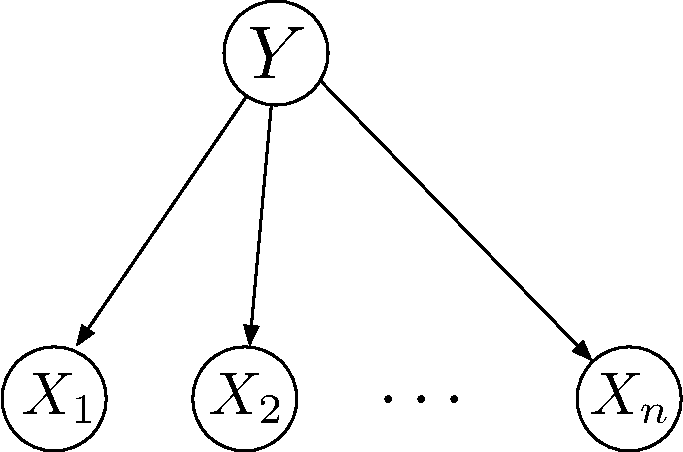
\includegraphics[width=\linewidth]{figures/naivebayesgm}
\end{marginfigure}


\section{Compas Model of Recidivism}


\end{document}
